\section{Implementation}
We implement our tool in JavaScript because we want our tool to be a web-based application, which can be easy to access. JavaScript also has a library called D3.js that is used for producing data visualization in web browsers. Our tool can be run in web browsers. We use the built-in HTTP server , \texttt{SimpleHTTPServer}, to test and run our tool. Next we describe UI components and other tools we use in order to implement our web-based application.
\subsection{UI Components}
Our tool consists of multiple UI components as follows:
\begin{itemize}
	\item \textbf{World Map Layer}: we use the geojson data~\cite{geocountries}, which contains information for each country, such as country polygon coordinates to draw the world map and ISO ALPHA-3 code.
	\item \textbf{HDI Map layer}: HDI Map layer is build on top of the world map layer, where we color each country polygon with different color based on how its HDI value ranked in all of the countries in our data set. As shown in Figure {fig: hdi}, countries with high HDI value will be colored bluer while countries with low HDI value will be colored redder.
	\begin{figure}[h!]
		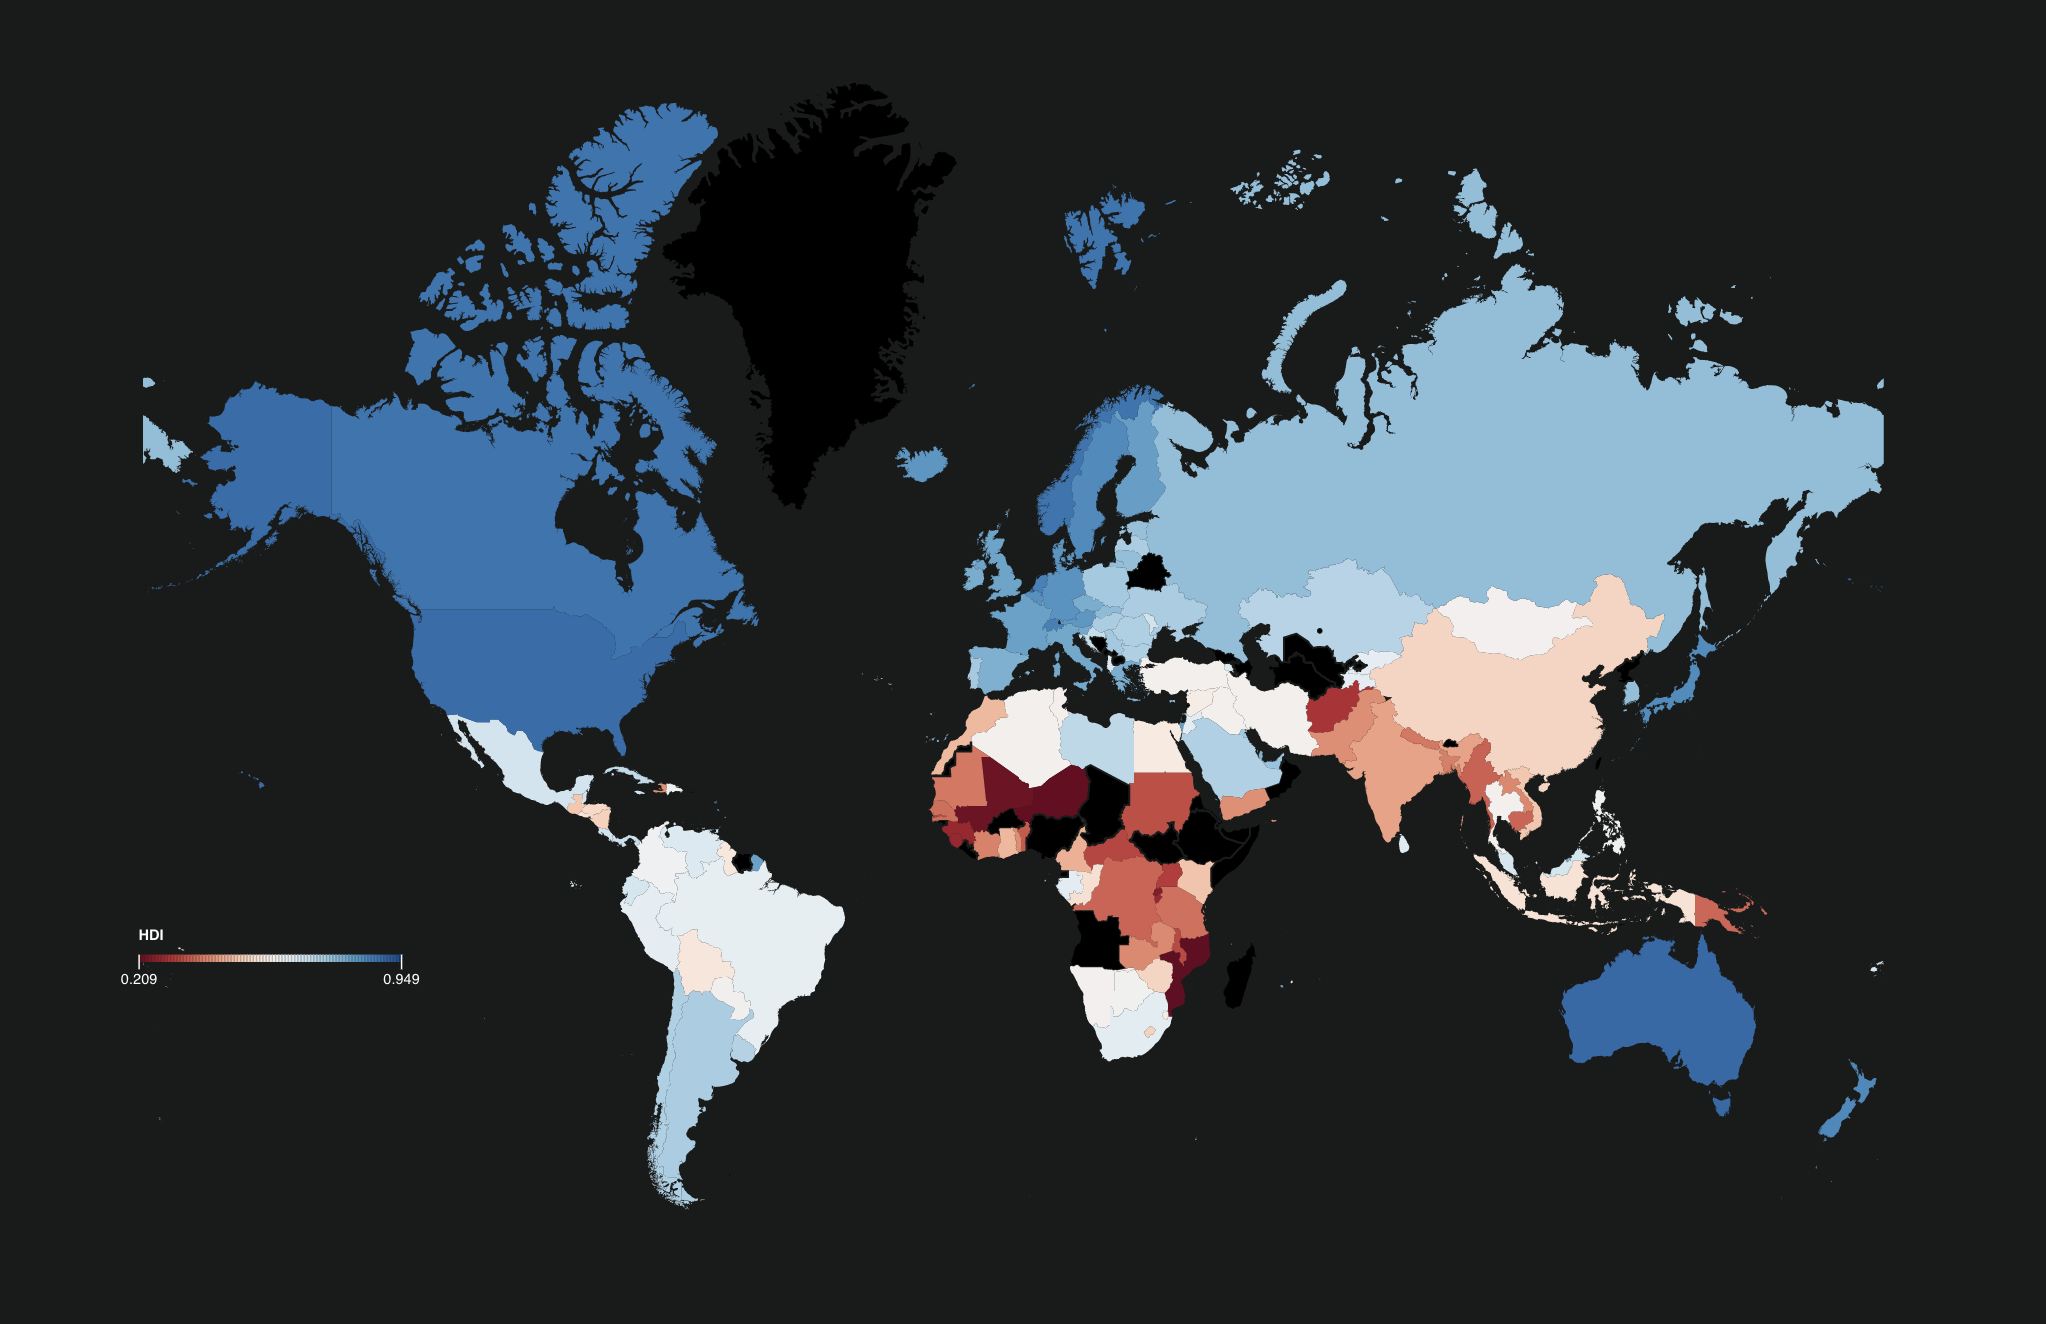
\includegraphics[width=0.4\textwidth]{hdiMap}
		\caption{HDI Map Layer}
		\label{fig:hdi}
	\end{figure}
	\item \textbf{Bivariate Map Layer}: Bivariate Map is also a type of color map. But instead of showing values in one field like HDI map layer, it compares two fields. The legend of bivariate map has two axises where there are three gradual colors for each axis and there will be nine colors in total. In our case, the bivariate map layer is been used to compare two components of HDI and it helps user to find any possible correlation between the two components. For example, in Figure \ref{fig: bivariate}, it shows that most of the countries in the world have a low value of GNI with a high value of expected year of school.
	\begin{figure}[h!]
		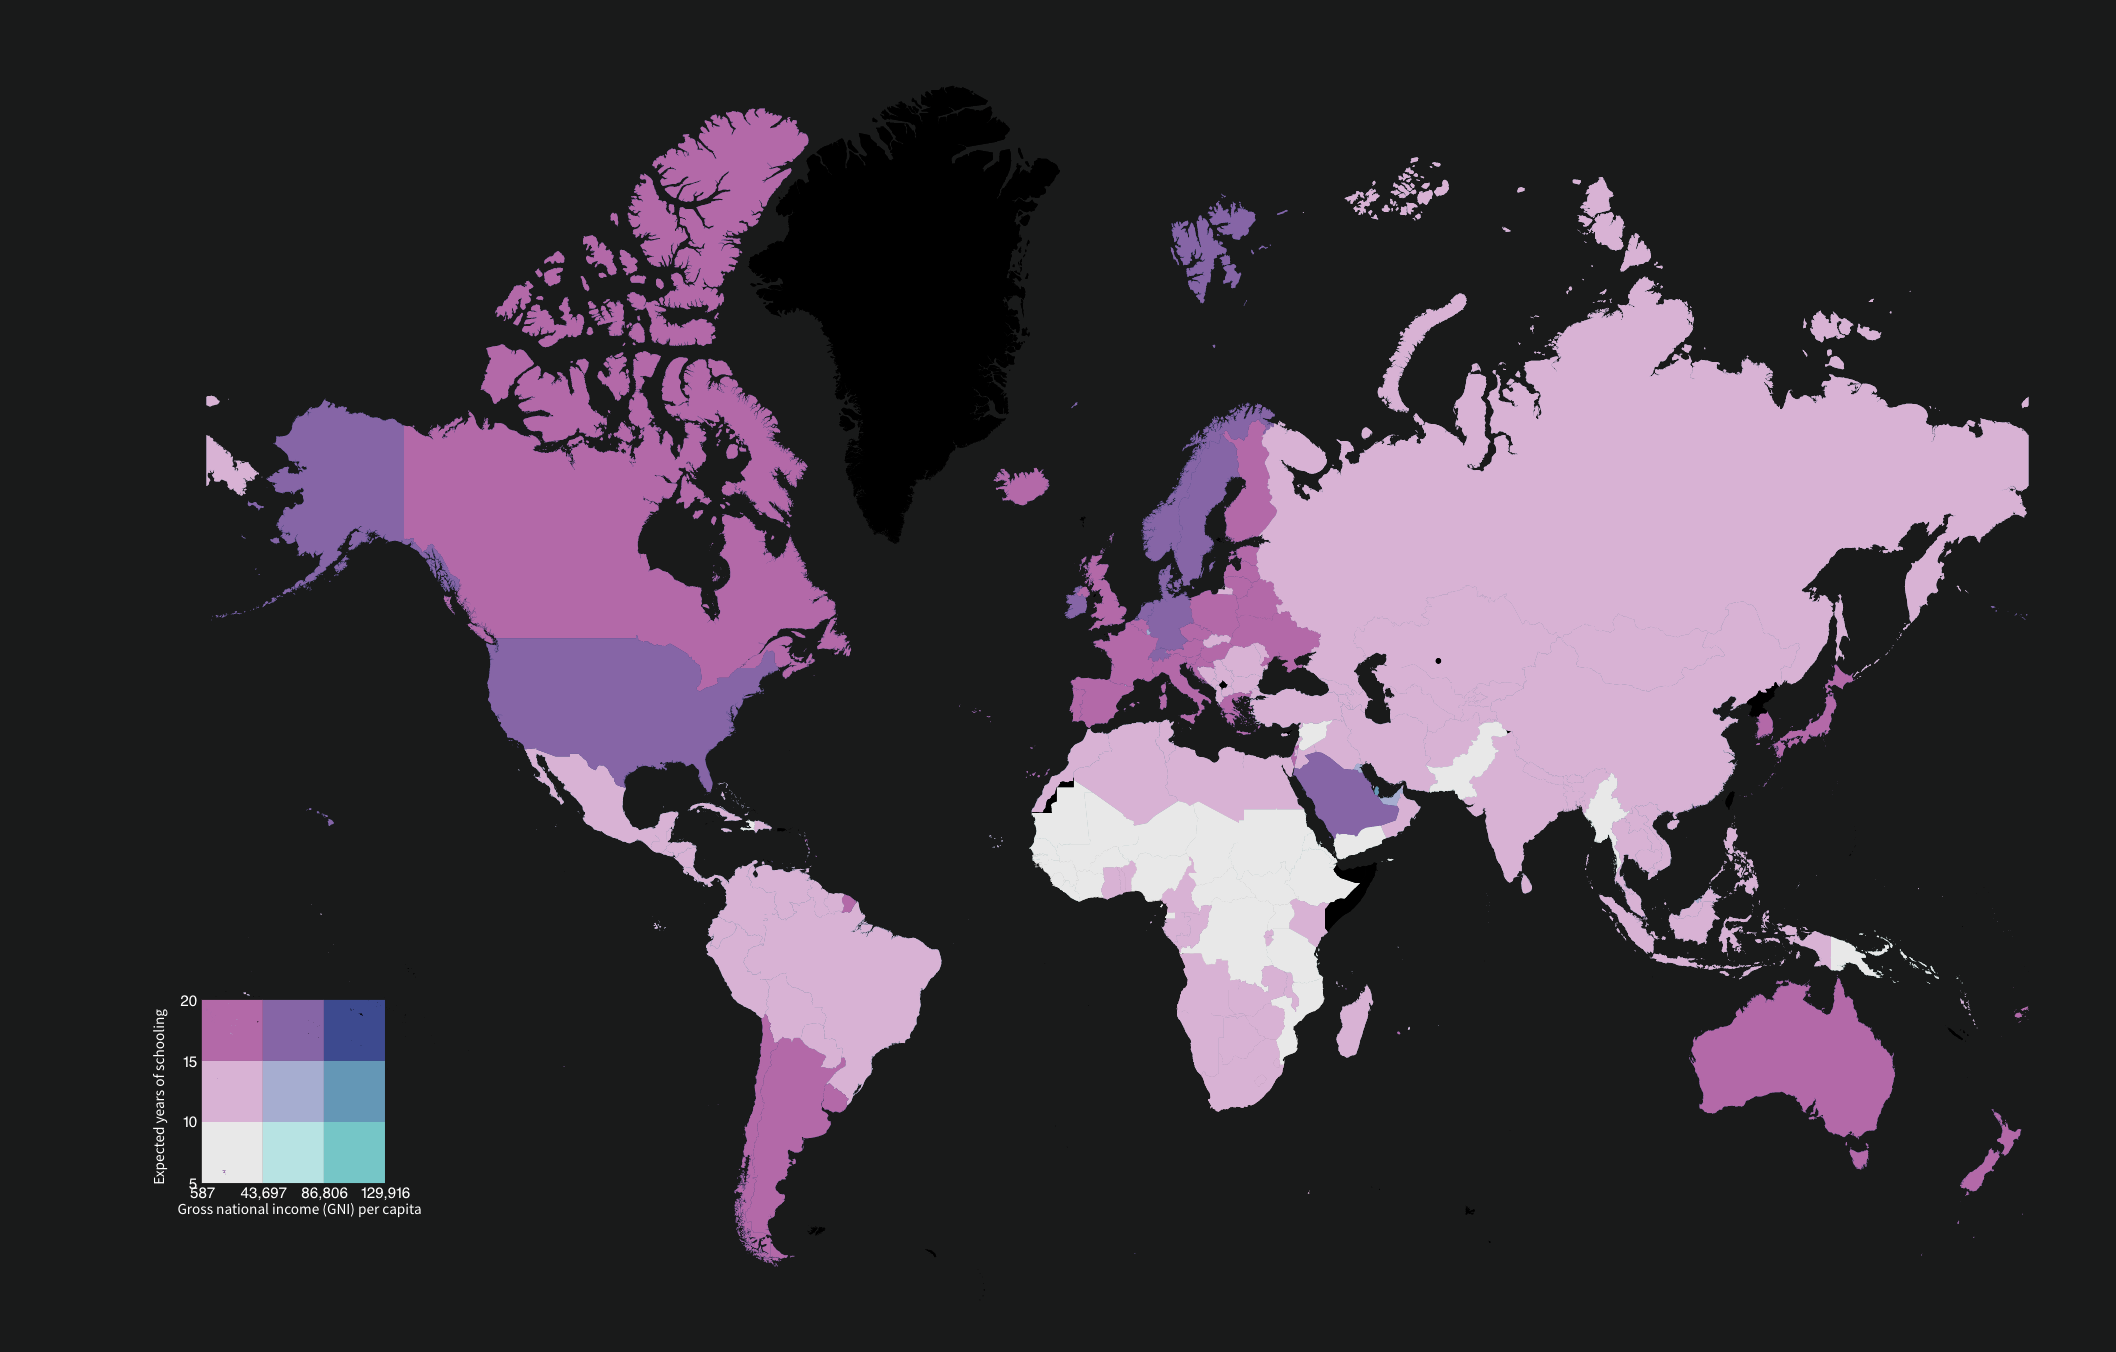
\includegraphics[width=0.4\textwidth]{bivariateMap}
		\caption{Bivaraite Map Layer}
		\label{fig:bivariate}
	\end{figure}
	\item \textbf{Parallel Coordinate Plot:} we use the parallel coordinate graph as a filter where the categorical x axis represents HDI and its components and each category on x axis will have one y axis. Then for each country, points will be plot along each y axis and connected together just as line chart. We allow user to brush on each y axis to select a range of data they are interested in. For instance, if the user is only interested in data with high HDI value and low GNI value, he can simply brush on y axises corresponds to those categories to filter out uninterested data. (Figure \ref{fig:parallel})
	\begin{figure}[h!]
		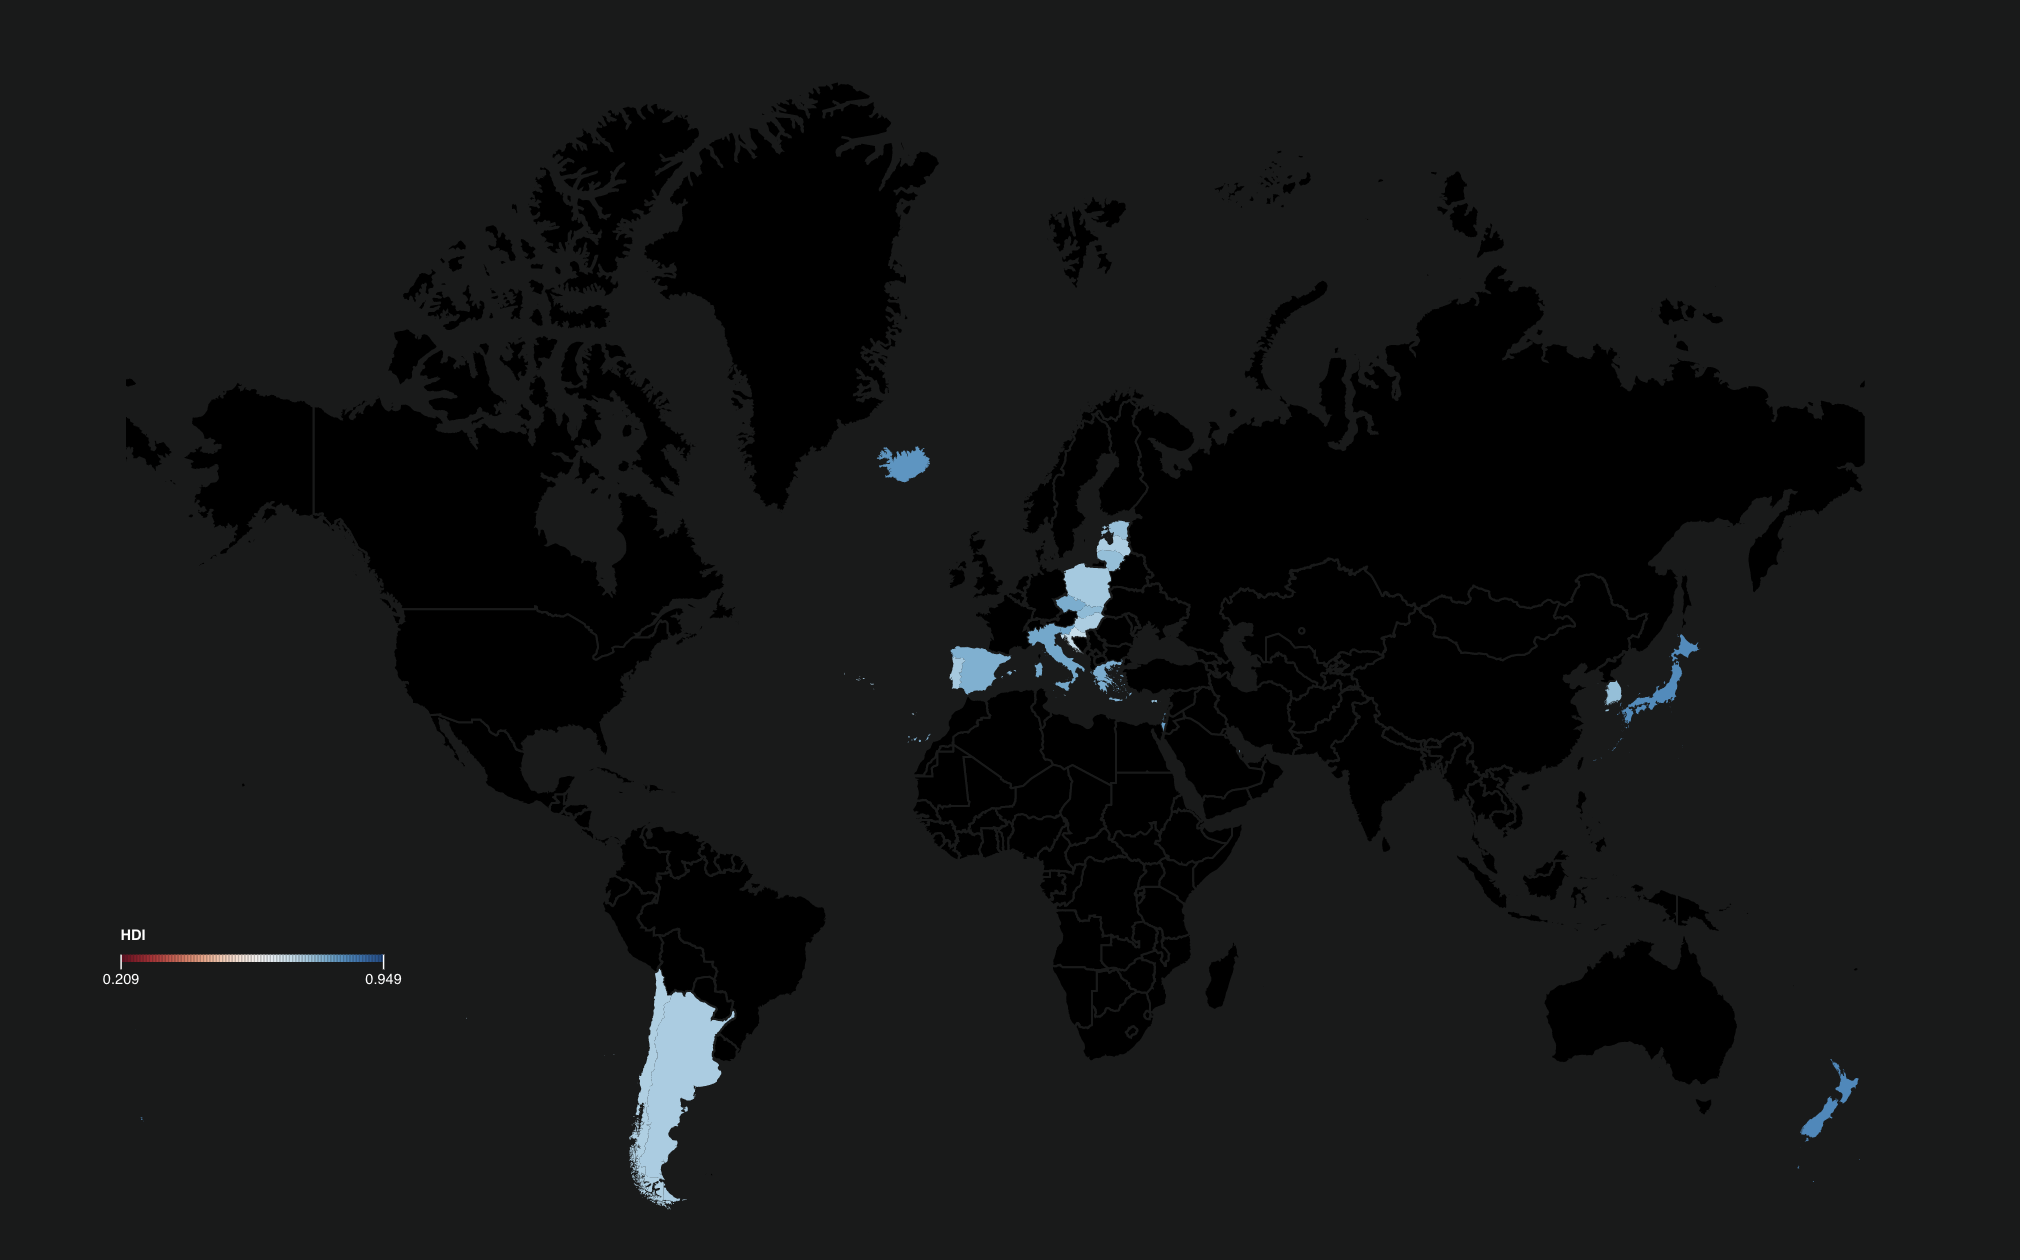
\includegraphics[width=0.4\textwidth]{filteredHdiMap}
		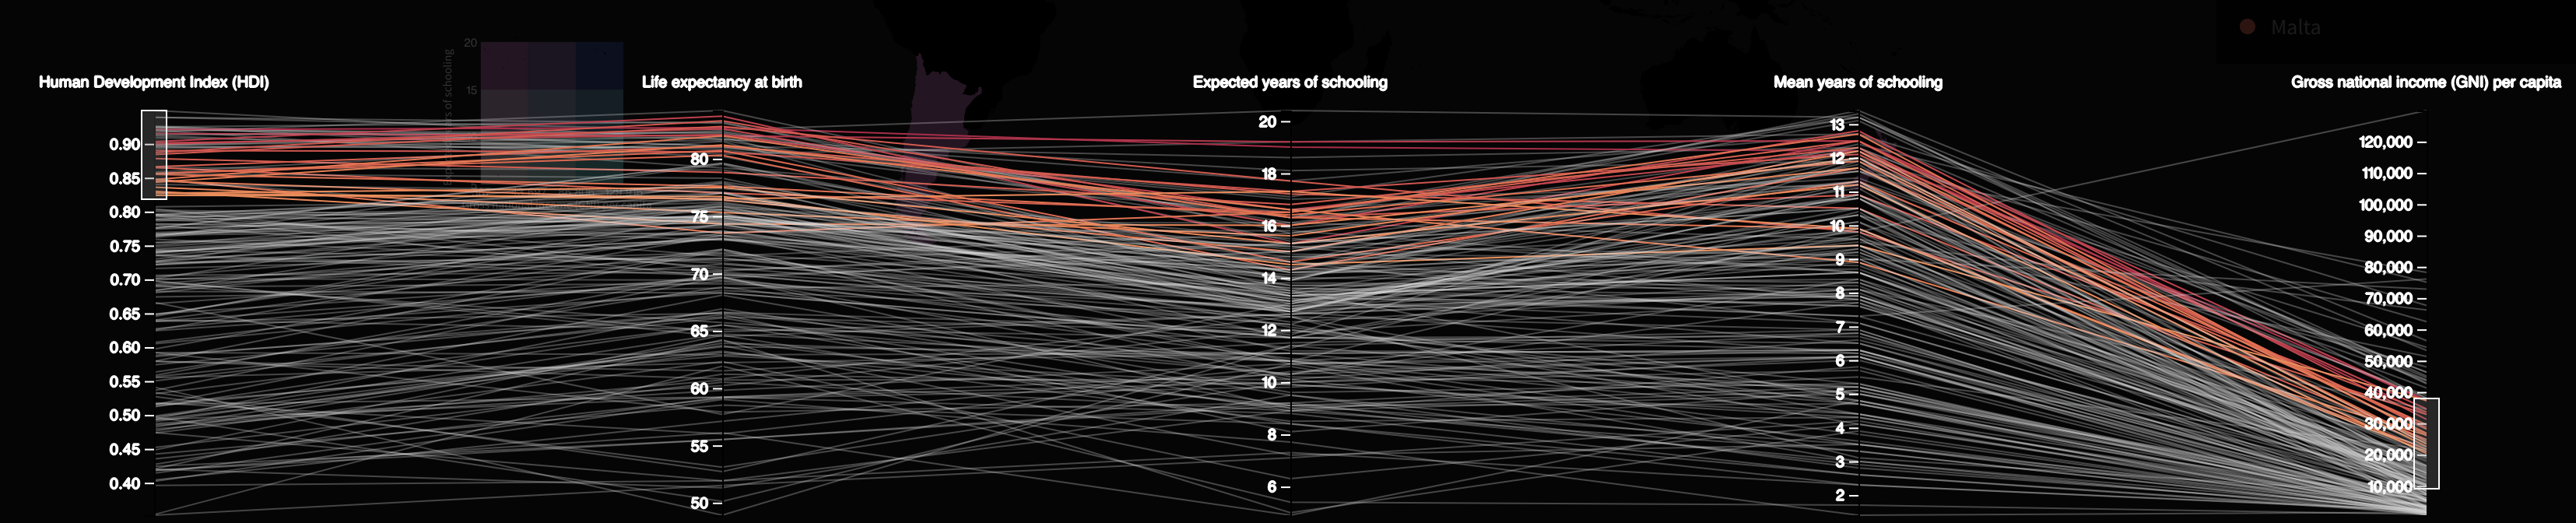
\includegraphics[width=0.4\textwidth]{parallelCoordGraph}
		\caption{filter countries with high HDI and low GNI}
		\label{fig:parallel}
	\end{figure}
	\item \textbf{Controller:} There three main components for the controller -- map selector, year slider and component selector. The map selector is responsible for deciding either the HDI map layer or the bivariate map layer will be shown. When the HDI map layer is shown, the year slider will appear as well that allow user to slide between 1990 and 2015. Correspondingly, the HDI map will show the data from different year, which provides a historical view of the HDI changes through years. When the multivariate map is selected, the year slider will be hidden and the component slider will be shown so that users can select the two components they are interested in to compare with. (figure \ref{fig:controller})
	\begin{figure}[h!]
		\centering
		\begin{subfigure}[b]{0.4\linewidth}
			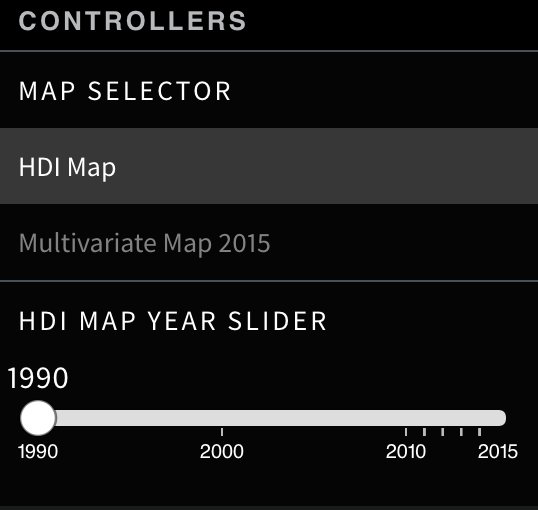
\includegraphics[width=\linewidth]{controllerHdi}
			\caption{select HDI map}
		\end{subfigure}
		\begin{subfigure}[b]{0.4\linewidth}
			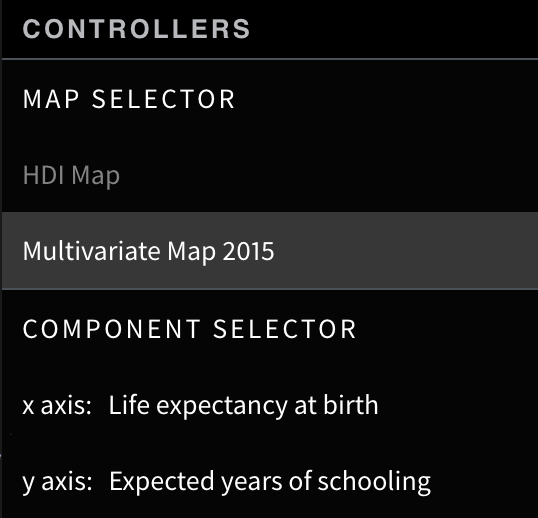
\includegraphics[width=\linewidth]{controllerBivariate}
			\caption{select Bivariate Map}
		\end{subfigure}
		\caption{Controller}
		\label{fig:controller}
	\end{figure}
    \item \textbf{Country Selector:} The country selector includes a search bar and a list of countries. The legend color next to the country name is corresponding to the color shown in the Parallel Coordinate Plot. When user start typing in the search bar, only countries with same starting letters as what user typed will be left in the list, which helps for user to find a specific country when they don't know where the country is actually located on the map. Also, when user can click on a country in the list, the corresponding country polygon on the map and corresponding country line in the parallel coordinate plot will be highlighted. The detailed information of the country will be show on the left side in the Country Info Panel.
    \item \textbf{Country Info Panel:} The panel will display detail information about the country selected either from the map or from the Country Selector. It contains two parts: statistics and spider graph. As shown in Figure xx, when the HDI map layer is shown,  the statistics are  HDI rank and value of the country; when the Bivariate map is shown, the statistics are the value of the two components of HDI. For the spider graph, it provides a straightforward view of the percentages of HDI and its components in all countries. It's easier for user to compare two countries than simple text because the similarity of two countries can be  represented by similar shapes.(Figure \ref{fig:panel})
    \begin{figure}[h!]
    	\centering
    	\begin{subfigure}[b]{0.4\linewidth}
    		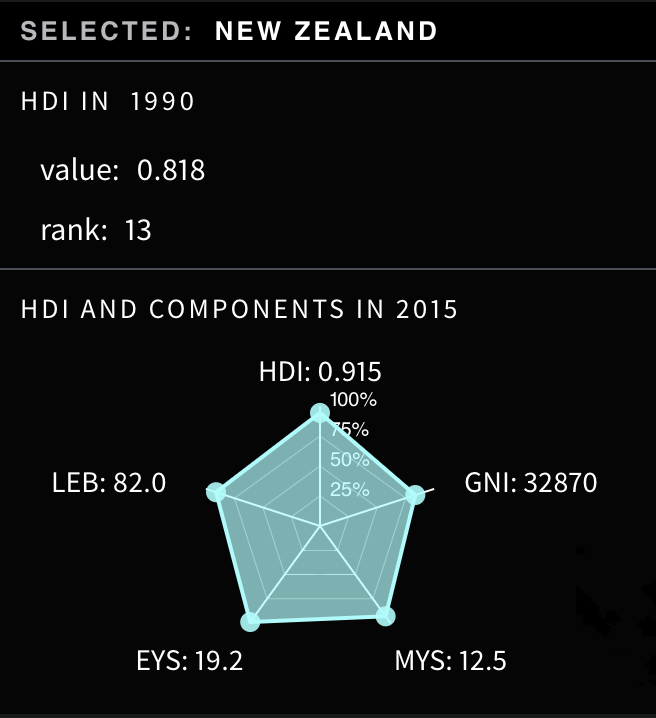
\includegraphics[width=\linewidth]{newZealand}
    		\caption{New Zealand}
    	\end{subfigure}
    	\begin{subfigure}[b]{0.4\linewidth}
    		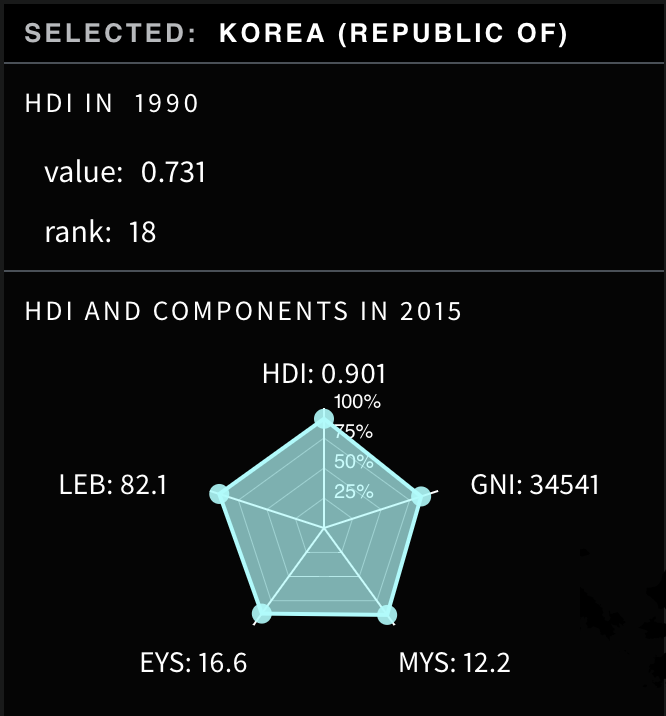
\includegraphics[width=\linewidth]{korea}
    		\caption{Korea}
    	\end{subfigure}
    	\caption{New Zealand and Korea has similar HDI rank and values of HDI components}
    	\label{fig:panel}
    \end{figure}
\end{itemize}

\subsection{Design Logic}
To creating the preceding UI components, we have a main html file that includes one HTML \texttt{<div>} wrapper with unique id for each UI component. And each UI component is been separated into a independent JS file as module, where we extract the corresponding wrapper div from main html to building visualizations. For charts and map, we use D3.js to create svg and inner layers. For communication between different UI components, we use d3.dispatch to generate event dispatchers and event listeners.  We also have a global js file that shares variables among all the components. As for styling, we created one css file for each component to independently manage style of components.
